\section{Benutzer Interface}



Konzepte, die hauptsächlich dazu dienen mit dem Spieler zu interagieren und sehr abhängig von seinen Entscheidungen sind.


\subsubsection{Kompass}
\begin{wrapfigure}{r}{0.4\textwidth}
  \begin{center}
    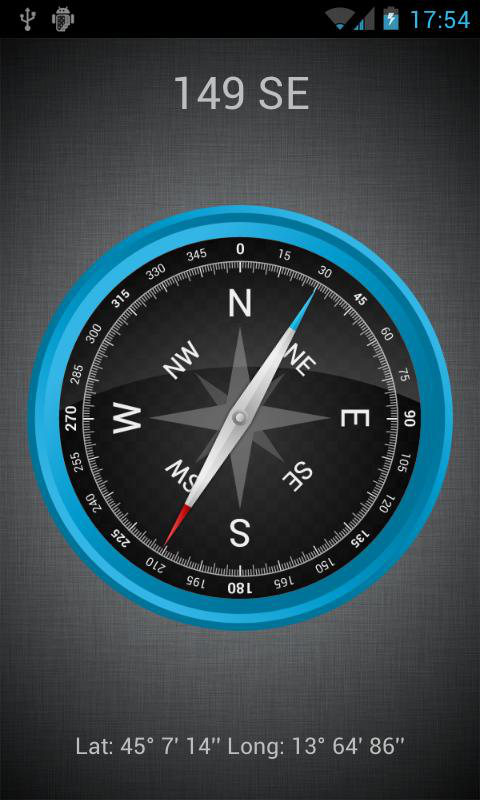
\includegraphics[width=0.3\textwidth]{3-Spielkonzepte/3-2-Benutzer_Interface/kompass.png}
     \caption{integrierter Kompass unter Android
	(Quelle: \url{https://lh6.ggpht.com/tQTY2Itaq9YtG8CZh8RA0N7sekCbURqBG5ZcpV6_u2no8Y8ezVIEibB4udVNFLzYKA\%3Dh900})
		}
  \end{center}
\end{wrapfigure}

Eine Richtungsangabe kann eine Karte ersetzen. Sei es um bei „Capture the Flag“ die
Richtung der Fahne des Gegners anzuzeigen oder für die „Snake“ das nächste
einzusammelnde Item. In der Regel hat es hier weniger Sinn, wenn die Kompassnadel nach
Norden zeigt.
\newline
Technische Lösungen:
Positionsermittlung (s. \ref{positionsermittlung}), GUI (s. \ref{gui}), Andere Sensorik (s. \ref{sensorik})

\subsubsection{Akustische und haptische Orientierungshilfen}

Akustische oder haptische Signale können ebenso Hinweise geben auf in der Nähe
befindliche Interessengebiete (z.B. ertönen eines Signals oder Vibration beim Erreichen eines
bestimmtem Umkreises von einem Item). 
Akustische oder haptische Signale können aber auch als Bestätigung eingesetzt
werden, wenn z.B. etwas eingesammelt wurde.
\newline
Technische Lösungen:
Kollisionsabfrage (s. \ref{kollisionsabfrage}), Andere Sensorik (s. \ref{sensorik})


\subsubsection{Geschwindigkeitsmessung}
Um das Spielgeschehen besser zu kontrollieren zu können, kann eine Messung der
Geschwindigkeit von Vorteil sein. Möchten wir z.B. bei Capute the Flag dem Fahnenträger
nicht erlauben eine gewissen Geschwindigkeit zu überschreiten, ist eine
Geschwindigkeitsmessung unabdingbar.
\newline
Technische Lösungen:
Positionsermittlung (s. \ref{positionsermittlung}), Server-Client-Kommunikation (s. \ref{kommunikation}), Andere Sensorik (s. \ref{sensorik})


\subsubsection{Mensch-Maschine-Kommunikation}
Das komplette Spielgeschehen lebt nach der Integrierung von mobilen Endgeräten von der Kommunikation zwischen Mensch und Gerät. Wird auf dem Endgerät ein Kompass angezeigt, muss der Spieler insofern reagieren, dass er sich in die richtige Richtung dreht.
Wenn er etwas einsammeln möchte, kann es erforderlich sein, dass ein Button gedrückt
wird.
\newline
Technische Lösungen:
GUI (s. \ref{gui}), Kartendarstellung (s. \ref{kartendarstellung})
